\chapter{Фильтрация и сортировка данных }
\section{Фильтрация данных с помощью предикатов }


Использование фильтров в запросе имеет значение и с точки зрения производительности. Прежде всего, выполняя фильтрацию строк в запросе (а не на клиенте),
мы снижаем нагрузку на сеть. Кроме того, учитывая информацию фильтров в запросе, SQL Server способен оценить возможность использования индексов для
эффективного получения данных без полного сканирования таблицы. Важно заметить, что для эффективного использования индекса предикат должен иметь форму,
известную как аргумент поиска (search argument, SARG).

Предикат в форме "столбец оператор значение" или "значение оператор столбец"
может быть аргументом поиска. Например, такие предикаты, как col1 = 10 и
col1 > 10, являются аргументами поиска. Манипулирование фильтруемыми столбцами в большинстве случаев не позволяет предикатам быть аргументами поиска.
Примером манипулирования фильтруемым столбцом может быть применение
к нему функции, скажем, F(col1) = 10, где F — некая функция. 

\begin{lstlisting}[label=lst:funcReturn,  language=sql]
	SELECT orderid, orderdate, empid
	FROM Sales.Orders
	WHERE COALESCE(shippeddate, '19000101') = COALESCE(@dt, '19000101');
\end{lstlisting}

Проблема заключается в том, что, хотя такой запрос возвращает правильный результат — даже в случае значения NULL на входе — предикат не является аргументом поиска. Это означает, что SQL Server не может эффективно использовать индекс для столбца shippeddate. Для того чтобы сделать предикат аргументом поиска,
следует избегать манипулирования фильтруемым столбцом и переписать предикат
следующим образом: 

\begin{lstlisting}[label=lst:funcReturn,  language=sql]
	SELECT orderid, orderdate, empid
	FROM Sales.Orders
	WHERE shippeddate = @dt
	OR (shippeddate IS NULL AND @dt IS NULL);
\end{lstlisting}

\begin{figure}[h!]
	\begin{center}
		
\includegraphics[width=1\textwidth]{img/advice3.png}
	\end{center}
	\captionsetup{justification=centering}
\end{figure}


В другом примере манипулирования фильтруемый столбец входит в выражение,
например, $col1 - 1 <= @n$. Иногда можно переписать предикат в форме, являющейся аргументом поиска, что сделает возможным эффективное использование индексирования. Например, последний предикат можно переписать с помощью простого
математического выражения $col1 <= @n + 1$.


\subsection{Предикат LIKE}


\begin{figure}[h!]
	\begin{center}
		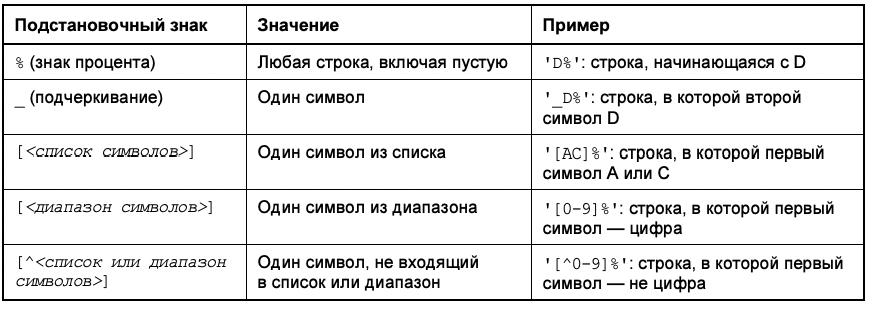
\includegraphics[width=1\textwidth]{img/like.png}
	\end{center}
	\captionsetup{justification=centering}
\end{figure}

\newpage
\begin{figure}[h!]
	\begin{center}
		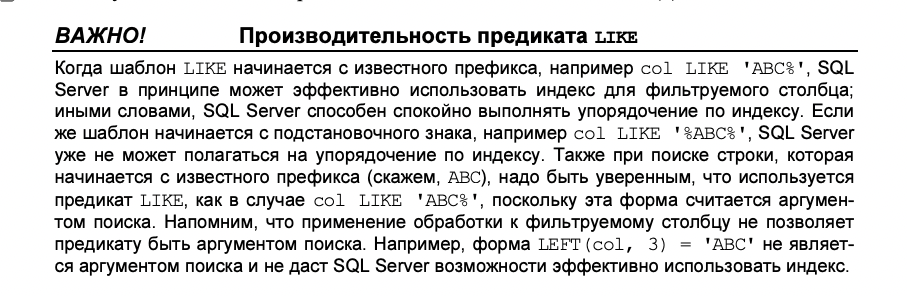
\includegraphics[width=0.9\textwidth]{img/advice4.png}
	\end{center}
	\captionsetup{justification=centering}
\end{figure}



\subsection{Фильтрация данных даты и времени}

Рекомендуется писать запрос подобно следующему: 

\begin{lstlisting}[label=lst:funcReturn, caption=Пример работы с фильтрацией даты, language=sql]
	SELECT orderid, orderdate, empid, custid
	FROM Sales.Orders
	WHERE orderdate = '20070212';
\end{lstlisting}


\begin{figure}[h!]
	\begin{center}
		
\includegraphics[width=1\textwidth]{img/advice5.png}
	\end{center}
	\captionsetup{justification=centering}
\end{figure}


Еще один важный аспект фильтрации данных даты и времени — постараться, когда это возможно, использовать аргументы поиска. Например, пусть нужно отфильтровать только заказы, размещенные в феврале 2007 года. Можно использовать функции YEAR и MONTH, как в следующем примере: 

\begin{lstlisting}[label=lst:funcReturn, caption=Пример работы с фильтрацией даты без аргумента поиска, language=sql]
	SELECT orderid, orderdate, empid, custid
	FROM Sales.Orders
	WHERE YEAR(orderdate) = 2007 AND MONTH(orderdate) = 2;
\end{lstlisting}

Однако поскольку в данном случае выполняются манипуляции с фильтруемым столбцом, предикат не может рассматриваться как аргумент поиска и, следовательно, SQL Server не сможет полагаться на упорядочение по индексу. Следует переписать этот предикат в виде диапазона, как показано в следующем примере: 

\begin{lstlisting}[label=lst:funcReturn, caption=Пример работы с фильтрацией даты с аргументом поиска, language=sql]
	SELECT orderid, orderdate, empid, custid
	FROM Sales.Orders
	WHERE orderdate >= '20070201' AND orderdate < '20070301';	
\end{lstlisting}

\begin{figure}[h!]
	\begin{center}
		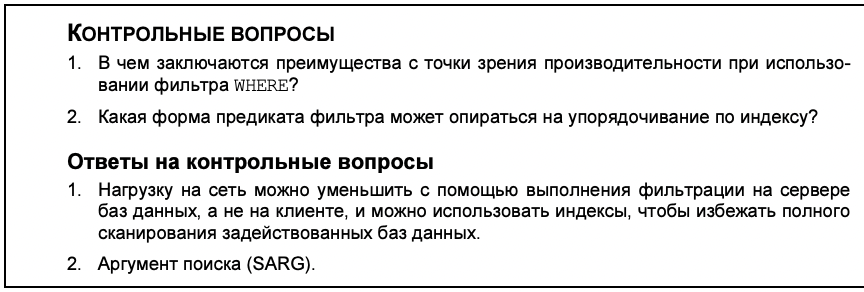
\includegraphics[width=0.9\textwidth]{img/control8.png}
	\end{center}
	\captionsetup{justification=centering}
\end{figure}

\subsection*{Резюме занятия}
\begin{itemize}
	\item Используя предложение WHERE, можно выполнять фильтрацию данных с помощью предикатов. Предикаты в языке T-SQL используют трехуровневую логику. Предложение WHERE возвращает случаи, когда предикат принимает значение <<истина>> и отбрасывает все прочие. 
	\item Фильтрация данных с предложением WHERE позволяет снизить нагрузку на сеть и
	может потенциально разрешать использование индексации для минимизации
	ввода-вывода. Для эффективного использования индексов важно представлять
	предикаты в виде аргументов поиска. 
\end{itemize}



\subsection*{Закрепление материала}

\begin{figure}[h!]
	\begin{center}
		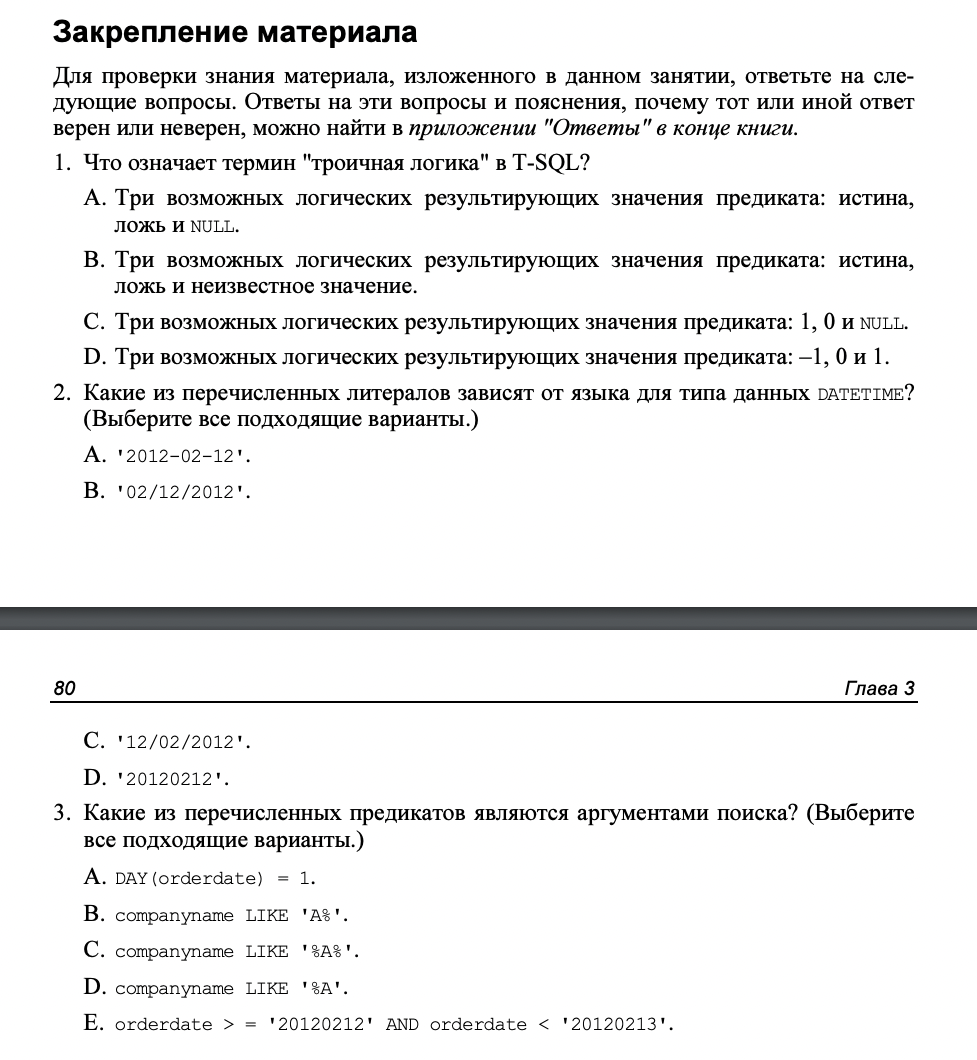
\includegraphics[width=0.9\textwidth]{img/zakrep5.png}
	\end{center}
	\captionsetup{justification=centering}
\end{figure}
\newpage

\subsection*{Ответы}

\begin{figure}[h!]
	\begin{center}
		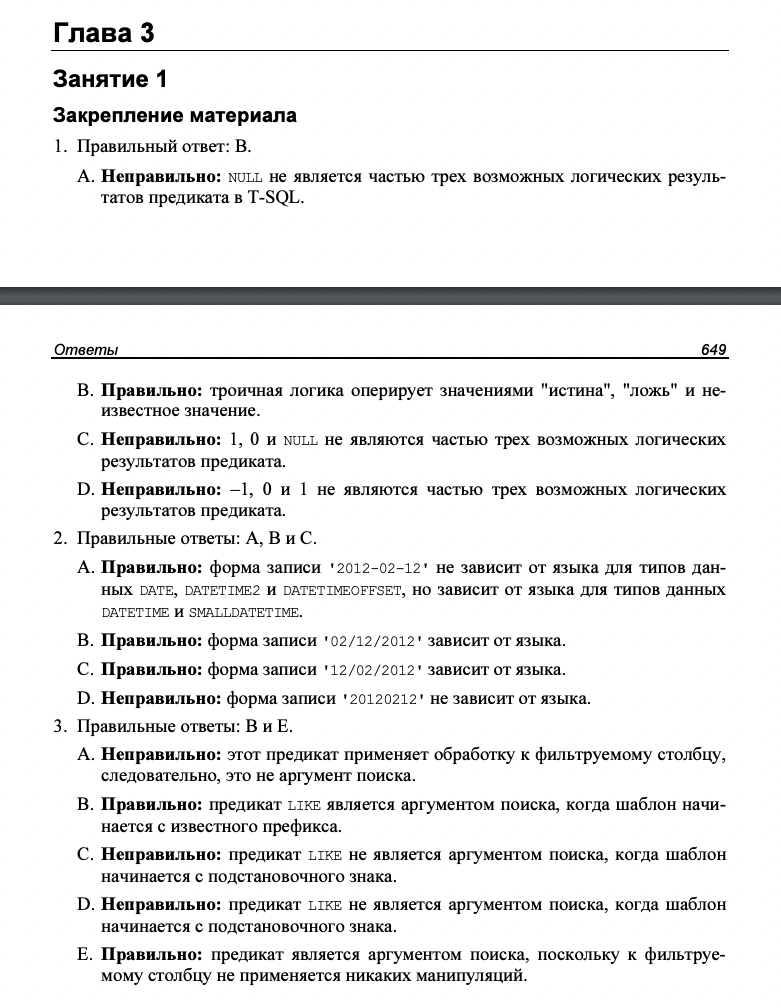
\includegraphics[width=0.9\textwidth]{img/ans5.png}
	\end{center}
	\captionsetup{justification=centering}
\end{figure}
\clearpage




\section{Сортировка данных}

\begin{figure}[h!]
	\begin{center}
		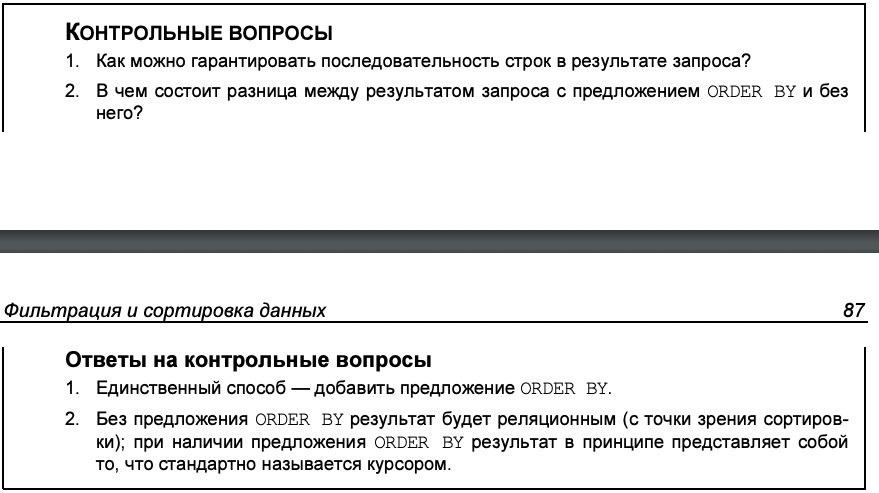
\includegraphics[width=0.9\textwidth]{img/control9.png}
	\end{center}
	\captionsetup{justification=centering}
\end{figure}




\subsection*{Резюме занятия}
\begin{itemize}
	\item Запросы, как правило, возвращают реляционный результат там, где сортировка
	не гарантирована. Если вам необходимо гарантировать упорядочение представления, нужно в запросе добавить предложение ORDER BY. 
	для манипулирования данными даты и времени, символьными строковыми данными и другими типами данных. Помните, что язык T-SQL в основном был
	предназначен для обработки данных, а не для форматирования или подобных
	задач. Таким образом, в этих областях, как правило, можно получить только
	базовую поддержку. Подобные задачи, как правило, лучше всего выполнять на
	клиенте. 
	\item С помощью предложения ORDER BY можно указать список выражений для первичной сортировки, вторичной сортировки и т. д. Для каждого выражения можно указать параметры ASC и DESC для упорядочения по возрастанию или убыванию, при этом по умолчанию принимается сортировка по возрастанию. 
	\item Даже если указано предложение ORDER BY, в результате все равно может получиться недетерминированная сортировка. Чтобы она была детерминированной,
	список ORDER BY должен быть уникальным.
	\item Можно использовать порядковые номера выражений из списка SELECT в предложении ORDER BY, но это считается плохой практикой. 
	\item Можно выполнять сортировку по элементам, появляющимся в списке SELECT,
	если предложение DISTINCT также не определено.
	\item Поскольку считается, что предложение ORDER BY обрабатывается после предложения SELECT, можно ссылаться на псевдонимы, присвоенные в предложении
	SELECT внутри предложения ORDER BY.
	\item При сортировке SQL Server считает значения NULL ниже, чем значения не-NULL, и
	равными друг другу. Это означает, что при упорядочивании по возрастанию они
	сортируются все вместе перед не-NULL-маркерами. 	
\end{itemize}


\subsection*{Закрепление материала}

\begin{figure}[h!]
	\begin{center}
		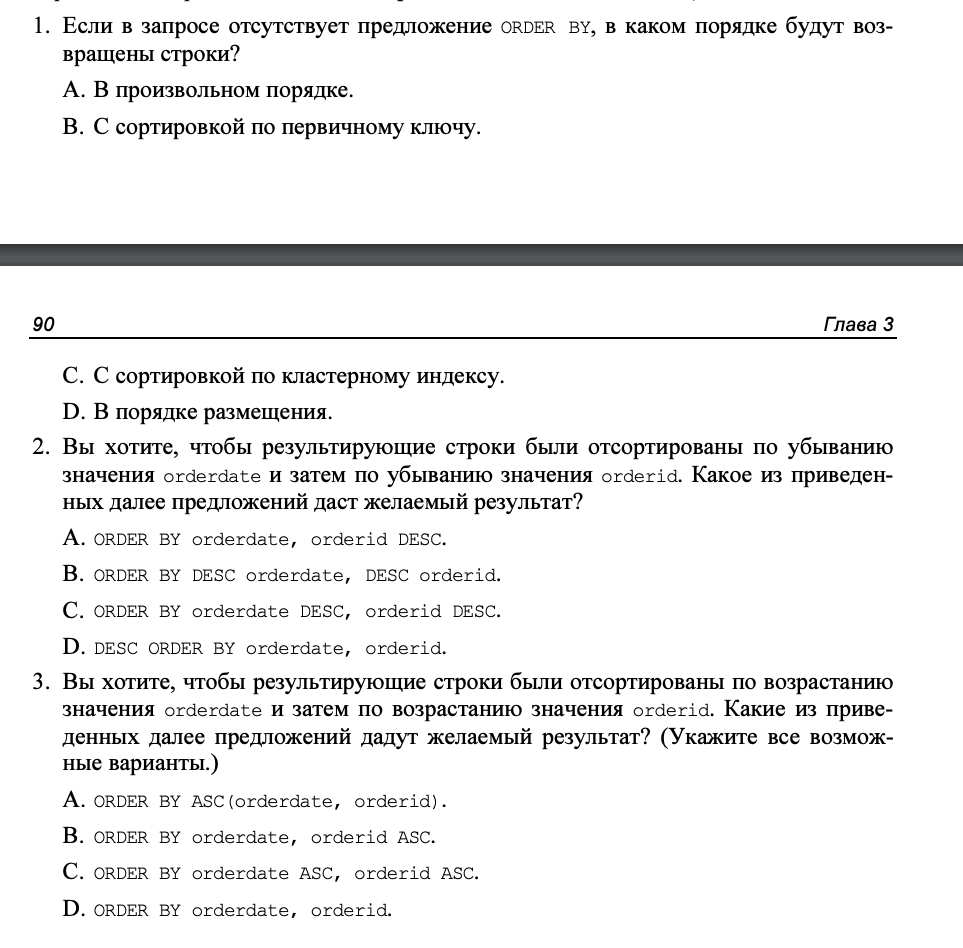
\includegraphics[width=0.9\textwidth]{img/zakrep6.png}
	\end{center}
	\captionsetup{justification=centering}
\end{figure}
\clearpage

\subsection*{Ответы}

\begin{figure}[h!]
	\begin{center}
		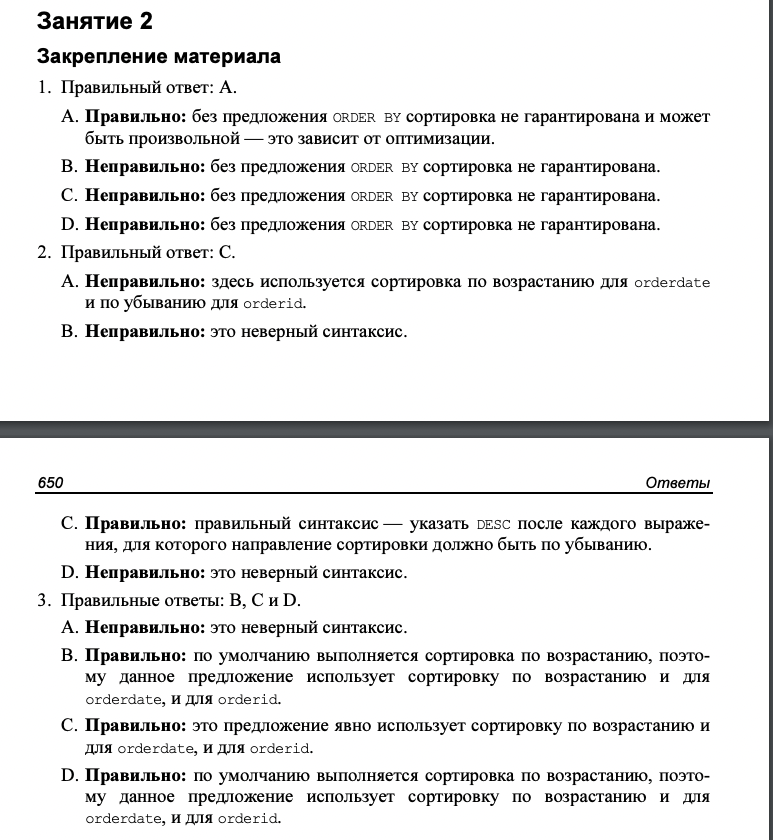
\includegraphics[width=0.9\textwidth]{img/ans6.png}
	\end{center}
	\captionsetup{justification=centering}
\end{figure}



\section{Фильтрация данных с помощью TOP и OFFSET...FETCH} 

\subsection{Фильтрация данных с помощью предложения TOP}

\begin{lstlisting}[label=lst:funcReturn, caption=Пример работы с TOP, language=sql]
	SELECT TOP (3) orderid, orderdate, custid, empid
	FROM Sales.Orders
	ORDER BY orderdate DESC; 
\end{lstlisting}



\begin{figure}[h!]
	\begin{center}
		
\includegraphics[width=0.9\textwidth]{img/advice6.png}
	\end{center}
	\captionsetup{justification=centering}
\end{figure}

Вместо числа строк можно также указать процентное соотношение строк, которые
надо отфильтровать. Для этого укажите величину FLOAT в диапазоне от 0 до 100
в скобках и ключевое слово PERCENT после скобок, как показано в следующем примере:


\begin{lstlisting}[label=lst:funcReturn, language=sql]
	SELECT TOP (1) PERCENT orderid, orderdate, custid, empid
	FROM Sales.Orders
	ORDER BY orderdate DESC; 
\end{lstlisting}

Параметр PERCENT задает следующую целую часть результирующего количества
строк, если это не целое число. В нашем примере без использования предожения
TOP количество строк в результирующем наборе равно 830. Фильтрация 1% дает
8,3, и следующая целая часть этого числа равна 9; следовательно, этот запрос возвратит 9 строк. 


Предложение TOP не ограничено постоянным вводом, наоборот, оно позволяет указывать произвольное выражение. С практической точки зрения эта возможность
особенно важна, когда необходимо передать параметр переменной в качестве входных данных, как в приведенном далее примере кода. 

\begin{lstlisting}[label=lst:funcReturn, language=sql]
	DECLARE @n AS BIGINT = 5;
	SELECT TOP (@n) orderid, orderdate, custid, empid
	FROM Sales.Orders
	ORDER BY orderdate DESC;
\end{lstlisting}

Однако этот запрос не является детерминированным. Он фильтрует 3 строки, но
без всякой гарантии, какие именно три строки будут возвращены. Вы в итоге получите любые 3 строки, которые SQL Server выбрал первыми, и это зависит от оптимизации. 

Мы не всегда заботимся о том, чтобы результат был детерминированным или
повторяемым, но если это необходимо, можно использовать две возможности. Одна — попросить включить все связи с последней строкой, добавив аргумент WITH
TIES, как на примере далее. 

\begin{lstlisting}[label=lst:funcReturn,  language=sql]
	SELECT TOP (3) WITH TIES orderid, orderdate, custid, empid
	FROM Sales.Orders
	ORDER BY orderdate DESC;
\end{lstlisting}

\subsection{Фильтрация данных с помощью OFFSET...FETCH}


Следующий запрос задает сортировку на основе даты заказа по убыванию, далее — идентификатора заказа по
убыванию, а затем он пропускает 50 строк и выбирает следующие 25 строк. 

\begin{lstlisting}[label=lst:funcReturn,  language=sql]
	SELECT orderid, orderdate, custid, empid
	FROM Sales.Orders
	ORDER BY orderdate DESC, orderid DESC
	OFFSET 50 ROWS FETCH NEXT 25 ROWS ONLY; 
\end{lstlisting}


С помощью предложений OFFSET и FETCH можно в качестве входных данных использовать выражения. Это очень удобно, когда требуется динамически вычислять
входные значения. Например, представьте, что вы реализуете возможность постраничного просмотра, где пользователю возвращается одна страница строк за один
раз. Пользователь отправляет вашей процедуре или функции в качестве входных
параметров номер страницы (@pagenum parameter) и размер страницы (@pagesize
parameter). Это означает, что вам нужно пропустить количество строк, равное
@pagenum минус 1, умноженное на @pagesize, и выбрать следующие @pagesize
строк. Реализовать это можно с помощью следующего кода (с использованием локальных переменных для простоты): 

\begin{lstlisting}[label=lst:funcReturn,  language=sql]
	DECLARE @pagesize AS BIGINT = 25, @pagenum AS BIGINT = 3;
	SELECT orderid, orderdate, custid, empid
	FROM Sales.Orders
	ORDER BY orderdate DESC, orderid DESC
	OFFSET (@pagenum - 1) * @pagesize ROWS FETCH NEXT @pagesize ROWS ONLY;
\end{lstlisting}

Поскольку конструкция OFFSET...FETCH является стандартной, а TOP — нет, в случаях, когда они логически эквивалентны, рекомендуется использовать более привычный. Кроме того, OFFSET...FETCH имеет преимущество перед параметром TOP — он
поддерживает возможность пропуска данных. Однако OFFSET...FETCH не поддерживает имеющиеся у TOP возможности, такие как PERCENT и WITH TIES. 


\begin{figure}[h!]
	\begin{center}
		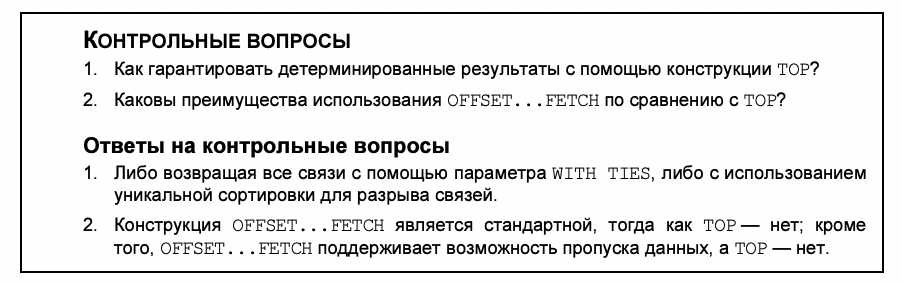
\includegraphics[width=0.9\textwidth]{img/control10.png}
	\end{center}
	\captionsetup{justification=centering}
\end{figure}

\subsection*{Практикум}


\begin{figure}[h!]
	\begin{center}
		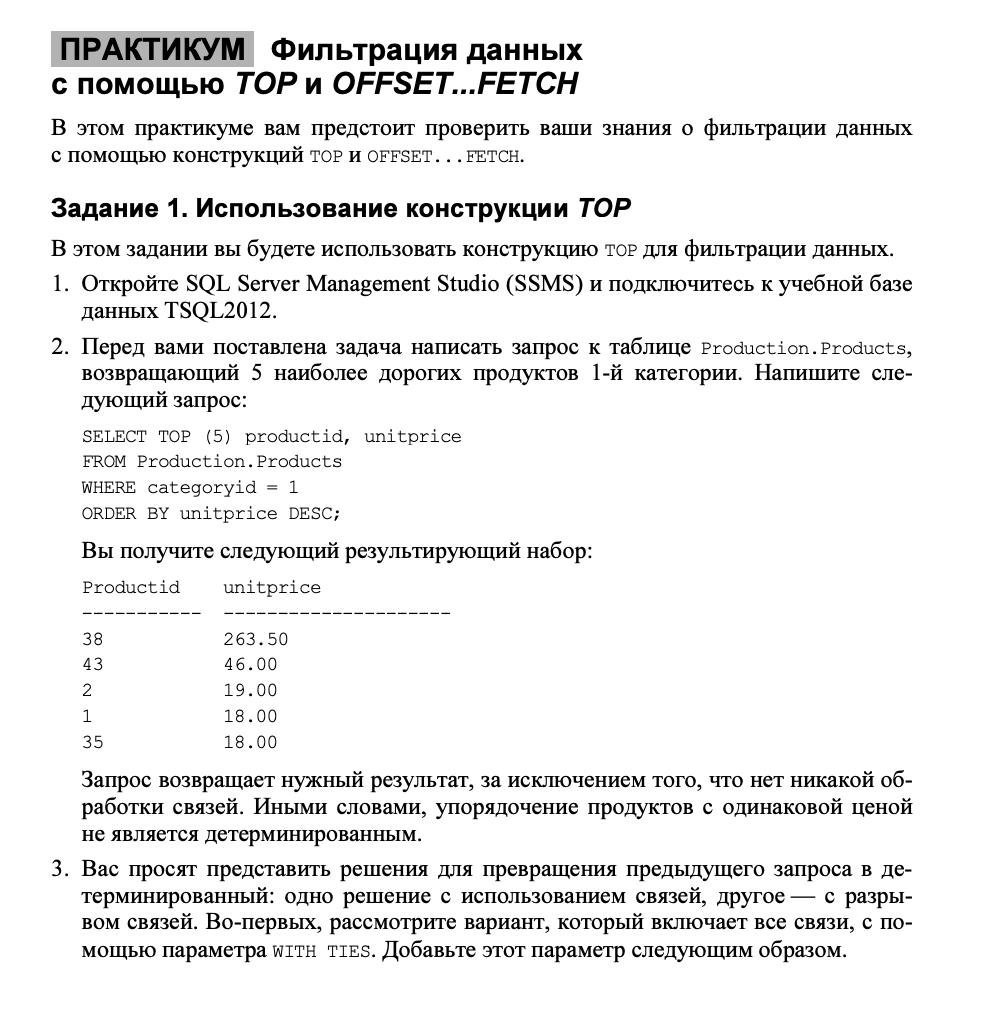
\includegraphics[width=0.9\textwidth]{img/ex3.png}
	\end{center}
	\captionsetup{justification=centering}
\end{figure}

\begin{figure}[h!]
	\begin{center}
		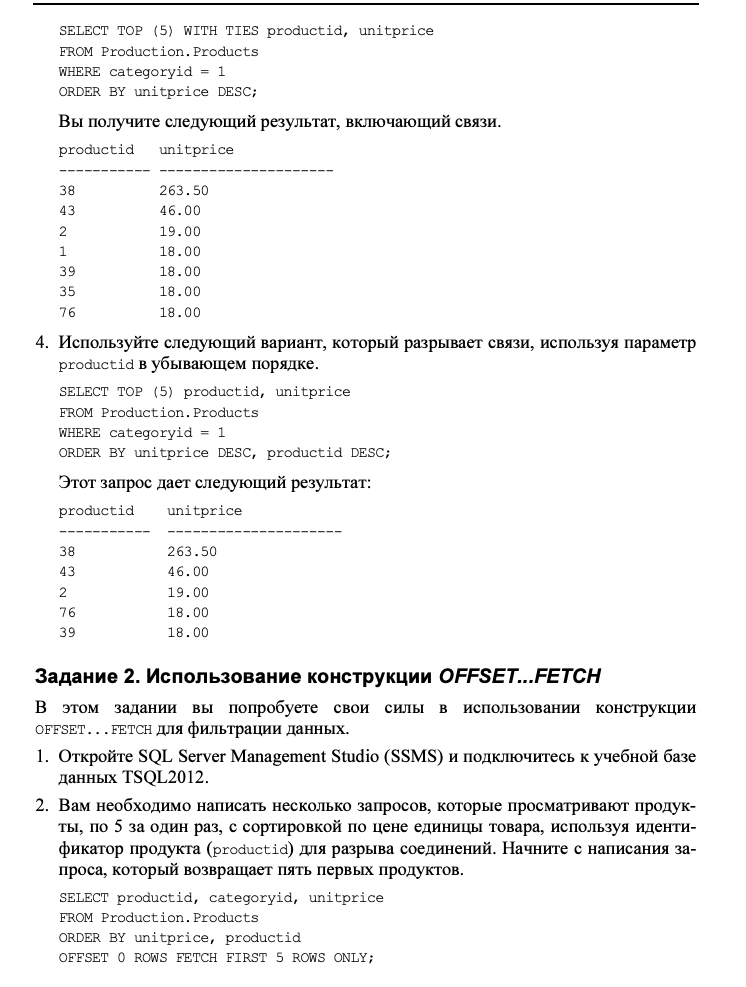
\includegraphics[width=0.9\textwidth]{img/ex4.png}
	\end{center}
	\captionsetup{justification=centering}
\end{figure}

\begin{figure}[h!]
	\begin{center}
		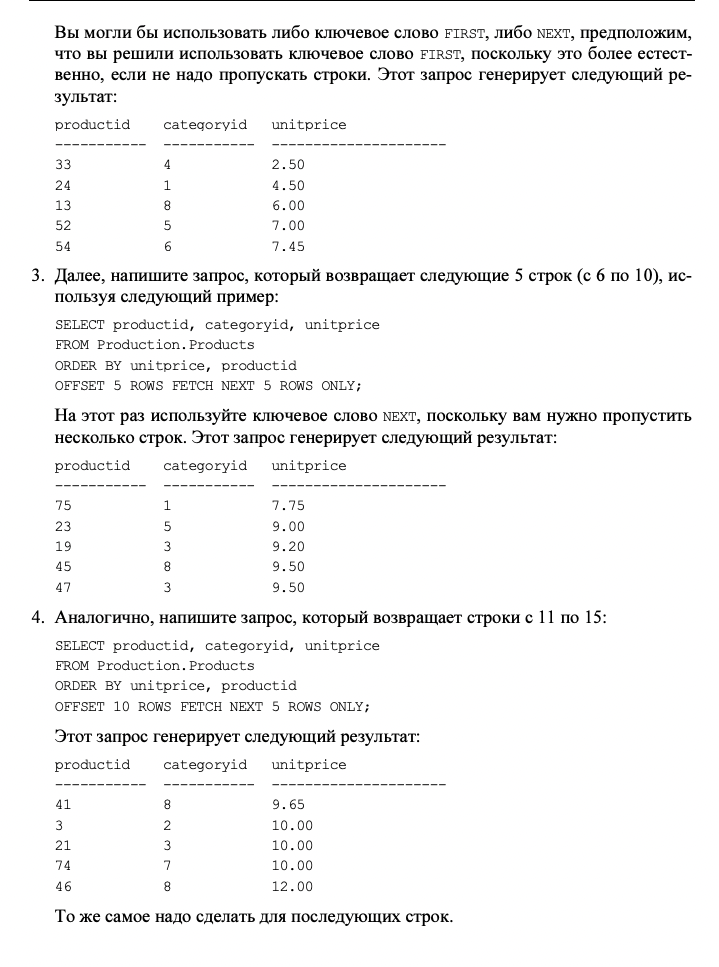
\includegraphics[width=0.9\textwidth]{img/ex5.png}
	\end{center}
	\captionsetup{justification=centering}
\end{figure}
\clearpage



\subsection*{Резюме занятия}
\begin{itemize}
	\item С помощью конструкций TOP и OFFSET...FETCH можно фильтровать даты на основе указанного количества строк и сортировки.
	\item Предложение ORDER BY, которое обычно используется в запросе для сортировки
	представления, также используется конструкциями TOP и OFFSET...FETCH, чтобы
	указать, какие строки надо фильтровать. 
	\item Параметр TOP — собственная возможность языка T-SQL, которую можно использовать для указания количества или процентного соотношения строк, подлежащих фильтрации. 
	\item Можно сделать запрос TOP детерминированным двумя способами: первый —
	используя параметр WITH TIES для возвращения всех связей, второй — используя
	уникальную сортировку для разрыва связей. 
	\item OFFSET...FETCH — это стандартная конструкция, подобная параметру TOP, поддерживаемая SQL Server 2012. В отличие от TOP она позволяет задать количество
	строк, которые надо пропустить, прежде чем указать число строк, которое следует отфильтровать. Поэтому она может использоваться для оперативной разбивки данных на страницы. 
	\item Как TOP, так и OFFSET...FETCH поддерживают в качестве входных данных выражения, а не только константы. 
\end{itemize}


\subsection*{Закрепление материала}

\begin{figure}[h!]
	\begin{center}
		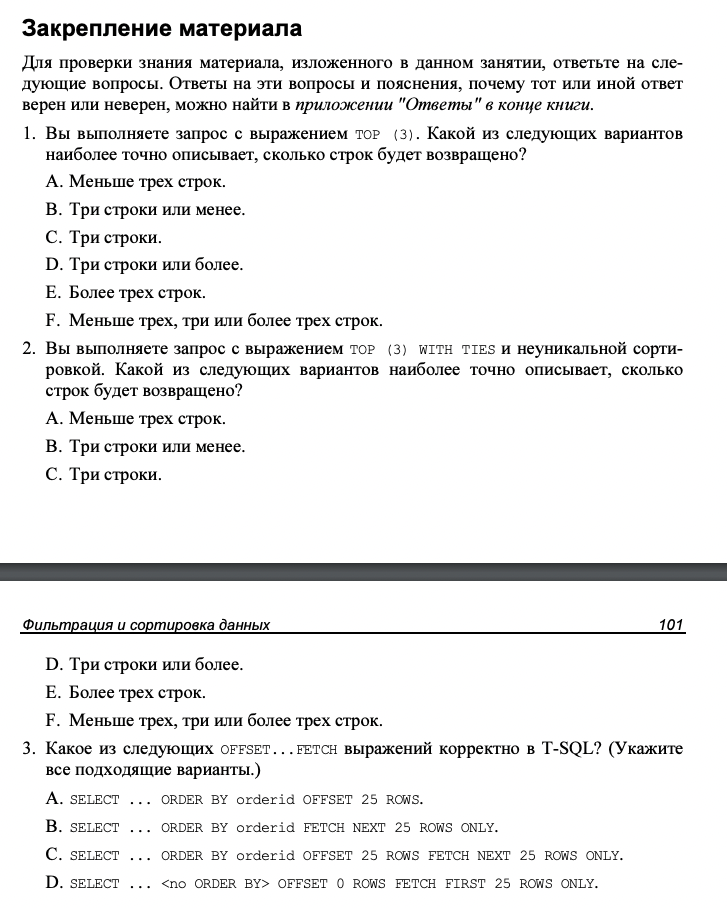
\includegraphics[width=0.9\textwidth]{img/zakrep7.png}
	\end{center}
	\captionsetup{justification=centering}
\end{figure}
\clearpage

\subsection*{Ответы}

\begin{figure}[h!]
	\begin{center}
		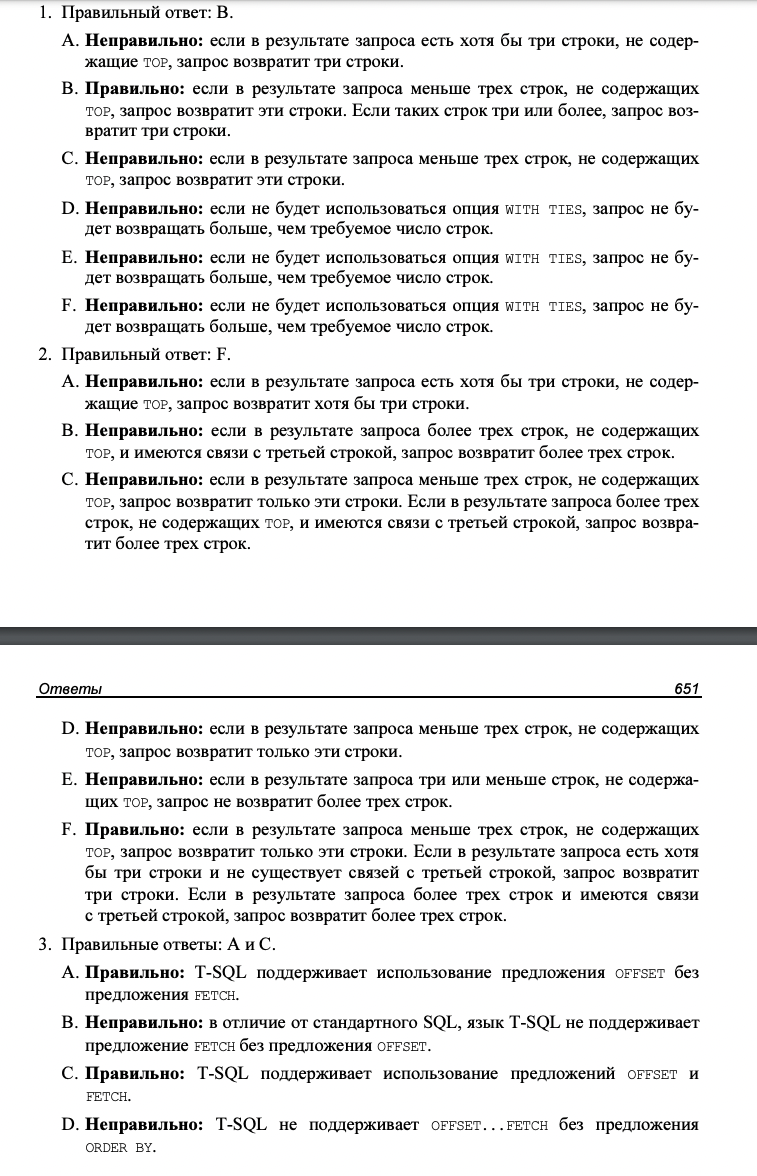
\includegraphics[width=0.8\textwidth]{img/ans7.png}
	\end{center}
	\captionsetup{justification=centering}
\end{figure}


\newpage
\subsection*{Упражнения}

\begin{figure}[h!]
	\begin{center}
		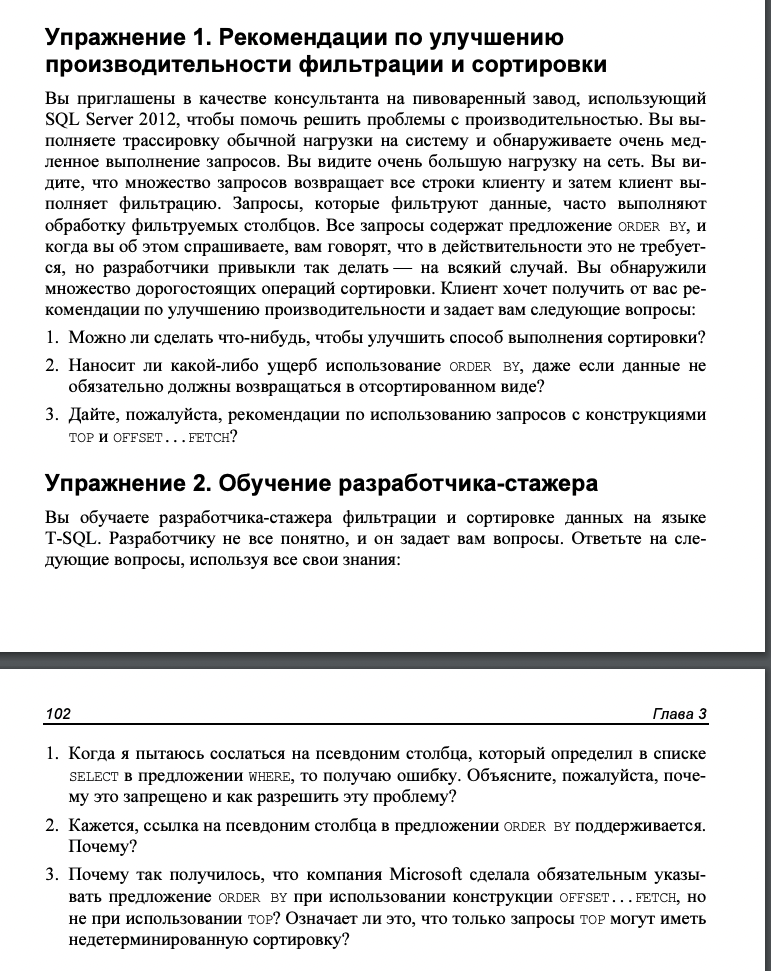
\includegraphics[width=0.9\textwidth]{img/ex6.png}
	\end{center}
	\captionsetup{justification=centering}
\end{figure}
\clearpage
\subsection*{Ответы}

\begin{figure}[h!]
	\begin{center}
		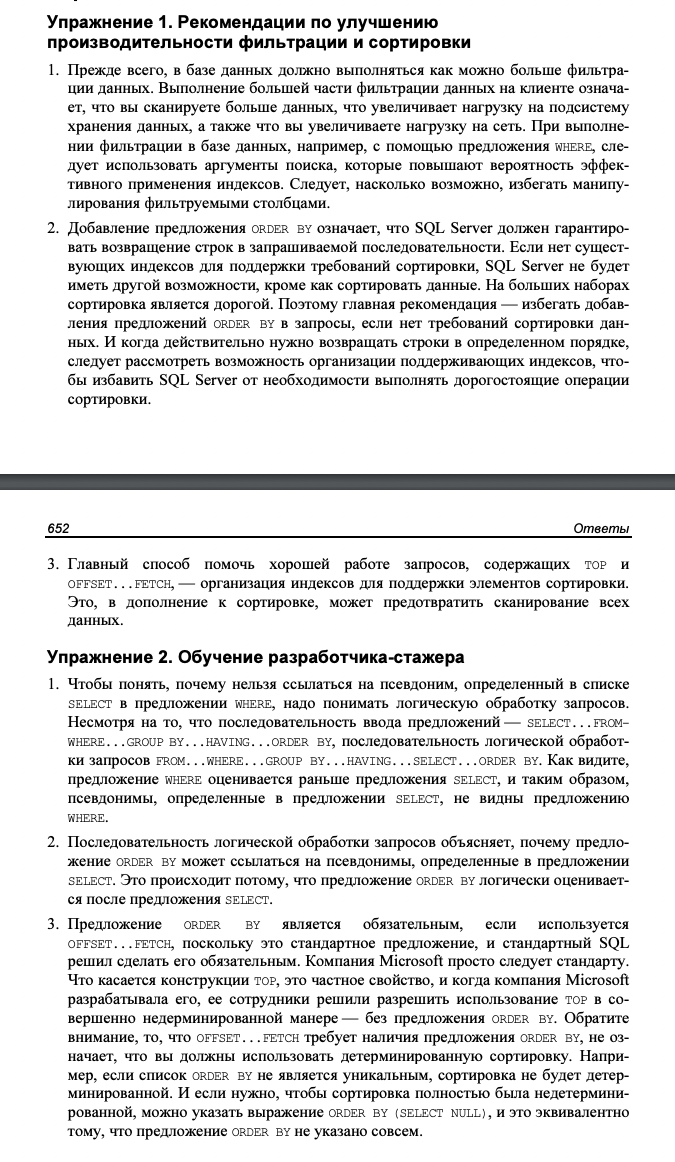
\includegraphics[width=0.7\textwidth]{img/eans3.png}
	\end{center}
	\captionsetup{justification=centering}
\end{figure}